\documentclass[aspectratio=169,11pt]{beamer}

\usepackage[T1]{fontenc}
\usepackage{lmodern}
\usepackage{amsmath,amssymb,bm}
\usepackage{graphicx}
\usepackage{booktabs}
\usepackage{tikz}
\usetikzlibrary{positioning,arrows.meta,shapes.geometric}
\usepackage{hyperref}

% -- Color palette: deep-space navy, cyan, and starlight gold --
\definecolor{SpaceNavy}{HTML}{10233E}
\definecolor{SpaceBlue}{HTML}{1D395B}
\definecolor{AstroCyan}{HTML}{007F96}
\definecolor{StarGold}{HTML}{E9AC50}
\definecolor{Ink}{HTML}{243344}
\definecolor{Mist}{HTML}{F3F7FA}
\definecolor{Muted}{HTML}{607487}

% -- Clean, modern Beamer appearance, no third-party themes --
\usetheme{default}
\usefonttheme{professionalfonts}
\setbeamertemplate{navigation symbols}{}
\setbeamertemplate{items}[circle]
\setbeamercolor{normal text}{fg=Ink,bg=white}
\setbeamercolor{frametitle}{fg=SpaceNavy,bg=white}
\setbeamerfont{frametitle}{size=\large,series=\bfseries}
\setbeamercolor{structure}{fg=AstroCyan}
\setbeamercolor{itemize item}{fg=AstroCyan}
\setbeamercolor{itemize subitem}{fg=AstroCyan}
\setbeamercolor{block title}{fg=white,bg=SpaceBlue}
\setbeamercolor{block body}{fg=Ink,bg=Mist}
\setbeamercolor{alerted text}{fg=AstroCyan}
\setbeamercolor{footline}{fg=Muted,bg=white}
\setbeamertemplate{frametitle}{%
  \vspace*{0.25cm}\insertframetitle\par
  \vspace*{0.06cm}{\color{AstroCyan}\rule{\linewidth}{0.65pt}}
}
\setbeamertemplate{footline}{%
  \ifnum\value{framenumber}>1
    \hspace{0.45cm}\scriptsize\textcolor{Muted}{\insertshortauthor\ \textbullet\ \insertshorttitle}
    \hfill\scriptsize\textcolor{Muted}{\insertframenumber\ / \inserttotalframenumber}\hspace{0.45cm}\vspace{0.20cm}
  \fi
}
\setbeamersize{text margin left=0.65cm,text margin right=0.65cm}

\title[Assessing AGN Light-Curves]{Bayesian Inference of\\AGN Light Curves}
\subtitle{Toward the identification of supermassive binary BHs}
\author[Julian Garlichs & Tim Zurbriggen]{Julian Garlichs and Tim Zurbriggen}
\date{\today}

\newcommand{\researchfigure}[2]{%
  \IfFileExists{#1}{%
    \includegraphics[width=\linewidth,height=#2,keepaspectratio]{#1}%
  }{%
    \begin{tikzpicture}
      \node[draw=AstroCyan!40,fill=Mist,rounded corners=3pt,
            minimum width=0.96\linewidth,minimum height=#2,align=center,
            text=Muted,inner sep=6pt] {%
        \normalsize Your figure goes here\\[4pt]
        \scriptsize\texttt{\detokenize{#1}}};
    \end{tikzpicture}%
  }%
}

\newcommand{\AGNbinarymotif}{%
  \begin{scope}[x=1cm,y=1cm]

    \begin{scope}[shift={(1.35,1.34)},rotate=-13]
      \fill[AstroCyan!17,opacity=0.7] (0,0) ellipse (0.74 and 0.24);
      \draw[AstroCyan!65,line width=0.70pt] (0,0) ellipse (0.74 and 0.24);
      \draw[AstroCyan!42,line width=0.48pt] (0,0) ellipse (0.55 and 0.16);
      \draw[AstroCyan!32,line width=1.45pt] (-0.69,0.0) arc[start angle=180,end angle=360,x radius=0.69,y radius=0.21];
      \draw[AstroCyan!95,line width=1.12pt] (0.68,0.02) arc[start angle=0,end angle=-180,x radius=0.68,y radius=0.21];
      \fill[SpaceNavy] (0,0) circle (0.145);
      \draw[white!70,line width=0.56pt] (0,0) circle (0.145);
    \end{scope}

    \begin{scope}[shift={(3.49,1.08)},rotate=-13]
      \fill[StarGold!15,opacity=0.70] (0,0) ellipse (0.61 and 0.19);
      \draw[StarGold!62,line width=0.70pt] (0,0) ellipse (0.61 and 0.19);
      \draw[StarGold!45,line width=0.48pt] (0,0) ellipse (0.43 and 0.125);
      \draw[StarGold!36,line width=1.35pt] (-0.56,0) arc[start angle=180,end angle=360,x radius=0.56,y radius=0.17];
      \draw[StarGold!95,line width=1.06pt] (0.56,0) arc[start angle=0,end angle=-180,x radius=0.56,y radius=0.17];
      \fill[SpaceNavy] (0,0) circle (0.105);
      \draw[white!70,line width=0.53pt] (0,0) circle (0.105);
    \end{scope}

    \node[anchor=west,text=white!56,font=\tiny] at (0.40,-0.34)
      {};
  \end{scope}%
}

% -- Section divider slide --
\newcommand{\sectiondivider}[1]{%
\begin{frame}[plain]
  \begin{tikzpicture}[remember picture,overlay]
    \fill[SpaceNavy] (current page.south west) rectangle (current page.north east);
    \draw[StarGold,line width=1.3pt]
      ([xshift=0.9cm,yshift=-2.1cm]current page.north west) -- ++(2.7cm,0);
    \node[anchor=west,text=white,font=\bfseries\LARGE]
      at ([xshift=0.9cm,yshift=-3.0cm]current page.north west) {#1};
    % Publication-style schematic, drawn as vector art.
    \begin{scope}[shift={([xshift=-5.2cm,yshift=0.85cm]current page.south east)},scale=0.96]
      \AGNbinarymotif
    \end{scope}
  \end{tikzpicture}
\end{frame}
}

\begin{document}

% Title
\begin{frame}[plain]
  \begin{tikzpicture}[remember picture,overlay]
    \fill[SpaceNavy] (current page.south west) rectangle (current page.north east);
    \node[anchor=west,text=AstroCyan!95!white,font=\bfseries\footnotesize]
      at ([xshift=0.9cm,yshift=-1.20cm]current page.north west)
      {Bayesian Statistics and Data Analysis};
    \draw[StarGold,line width=1.2pt]
      ([xshift=0.9cm,yshift=-1.48cm]current page.north west) -- ++(5.8cm,0);
    \node[anchor=west,text=white,text width=10.8cm,font=\bfseries\LARGE,align=left]
      at ([xshift=0.9cm,yshift=-2.93cm]current page.north west) {\inserttitle};
    \node[anchor=west,text=white!78,text width=10.6cm,font=\normalsize]
      at ([xshift=0.9cm,yshift=-4.02cm]current page.north west) {\insertsubtitle};
    % Scientifically styled binary-AGN illustration (not to scale).
    \begin{scope}[shift={([xshift=-5.1cm,yshift=0.90cm]current page.south east)},scale=0.97]
      \AGNbinarymotif
    \end{scope}
    \node[anchor=west,text=white!90,text width=8.9cm,font=\small]
      at ([xshift=0.9cm,yshift=1.10cm]current page.south west)
      {\insertauthor\quad | \quad \insertinstitute};
    \node[anchor=west,text=white!65,font=\scriptsize]
      at ([xshift=0.9cm,yshift=0.64cm]current page.south west) {\insertdate};
  \end{tikzpicture}
\end{frame}

\begin{frame}{Motivation}
  \vspace{0.10cm}
  \begin{block}{Scientific motivation}
    Supermassive binary black holes are thought to be common in the Universe as natural products of galaxy mergers and thus are probes of our current understanding. 
  \end{block}
  \vspace{0.16cm}
  \begin{columns}[T,onlytextwidth]
    \begin{column}{0.48\textwidth}
      \textbf{Challenges}
      \begin{itemize}
        \item Irregularly sampled fluxes
        \item Photometric uncertainties
        \item Long-term correlated variability
      \end{itemize}
    \end{column}
    \begin{column}{0.48\textwidth}
      \textbf{What we infer}
      \begin{itemize}
        \item Stochastic-process parameters
        \item Evidence for additional variability
        \item Posterior uncertainties
      \end{itemize}
    \end{column}
  \end{columns}
  \vfill
  {\small\color{Muted}A periodic-looking light curve is not, by itself, evidence for a binary SMBH.}
\end{frame}

\section{Background}
\sectiondivider{Background and Modeling}

\begin{frame}{Physical Background}


\begin{columns}[T,onlytextwidth]
    \begin{column}{0.66\textwidth}
      \centering
      \researchfigure{figures/data_model.pdf}{4.85cm}
    \end{column}
    \begin{column}{0.31\textwidth}
       Active galactic nucleis (AGNs) are active supermassive black holes at the center of galaxies that emit electromagnetic radiation as dust and gas falls into them. 
    \end{column}
  \end{columns}
  \vspace{0.05cm}
  {\scriptsize\color{Muted}Figure: Observed Light Curve of ... using ZTF data.}
    
\end{frame}

\begin{frame}{Bayesian Inference}
  Assuming stationary Gaussian noise, the likelihood function for a quasar light curve is

  \begin{equation*}
      \boxed{\displaystyle\mathcal{L}(\mathbf{d}| \Vec{\theta}_n, \Vec{\theta}_s, m) = \frac{1}{\sqrt{(2\pi)^N |\mathbf{C}|}} \exp \left[ -\frac{1}{2} (\mathbf{d - m - s})^\top \mathbf{C}^{-1} (\mathbf{d - m - s)} \right]}
  \end{equation*}

  where 
  \begin{itemize}
      \item $\mathbf{d}$ is time-series light curve data of length $N$
      \item $\Vec{\theta}_n$ and $\Vec{\theta}_s$ are our model parameters and include noise and signal parameters respectively
  \end{itemize}
  
\end{frame}

\begin{frame}{Bayesian Inference}
  Assuming stationary Gaussian noise, the likelihood function for a quasar light curve is

  \begin{equation*}
      \boxed{\displaystyle\mathcal{L}(\mathbf{d}| \Vec{\theta}_n, \Vec{\theta}_s, m) = \frac{1}{\sqrt{(2\pi)^N |\mathbf{C}|}} \exp \left[ -\frac{1}{2} (\mathbf{d - m - s})^\top \mathbf{C}^{-1} (\mathbf{d - m - s)} \right]}
  \end{equation*}

  We model $\mathbf{d}$ as

  \begin{equation*}
      \mathbf{d = n + m + s}
  \end{equation*}

  wehre $\mathbf{n}$ is the noise vector, $\mathbf{m}$ accounts for the mean magnitude and $\mathbf{s}$ is the signal vector defined as 

  \begin{equation*}
      \mathbf{s}(t) = A\sin (2\pi f_0 t + \phi).
  \end{equation*}
  
\end{frame}

\begin{frame}{From AGN variability to inference}
  \vspace{0.43cm}
  \centering
  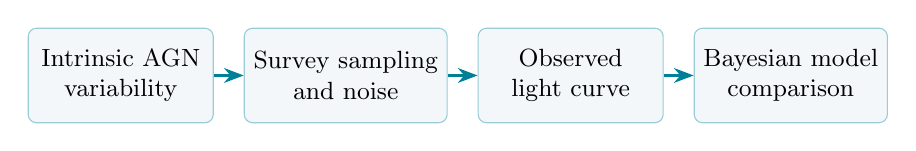
\begin{tikzpicture}[
    node distance=0.38cm,
    every node/.style={font=\small},
    box/.style={draw=AstroCyan!40,fill=Mist,rounded corners=3pt,
                minimum width=2.35cm,minimum height=1.2cm,align=center},
    arr/.style={-{Stealth[length=2.5mm]},line width=1pt,draw=AstroCyan}
  ]
    \node[box] (var) {Intrinsic AGN\\variability};
    \node[box,right=of var] (sampling) {Survey sampling\\and noise};
    \node[box,right=of sampling] (data) {Observed\\light curve};
    \node[box,right=of data] (infer) {Bayesian model\\comparison};
    \draw[arr] (var) -- (sampling);
    \draw[arr] (sampling) -- (data);
    \draw[arr] (data) -- (infer);
  \end{tikzpicture}
  \vfill
  \begin{block}{Key challenge}
    
  \end{block}
\end{frame}


\section{Methods}
\sectiondivider{Data \& Methods}

\begin{frame}{Data and Bayesian workflow}
  \begin{columns}[T,onlytextwidth]
    \begin{column}{0.49\textwidth}
      \textbf{Light-curve dataset}
      \begin{itemize}
        \item Survey: \emph{[e.g., ZTF]}
        \item Sources: \emph{[AGN selection]}
        \item Cadence and baseline: \emph{[values]}
        \item Quality cuts and uncertainties
      \end{itemize}
    \end{column}
    \begin{column}{0.49\textwidth}
      \textbf{Inference pipeline}
      \begin{enumerate}
        \item Choose stochastic / periodic models
        \item Construct the likelihood
        \item Set priors and sample posteriors
        \item Check convergence and predictive fit
        \item Compare model evidences
      \end{enumerate}
    \end{column}
  \end{columns}
  \vspace{0.18cm}
  \begin{block}{Bayes' theorem and marginal likelihood}
    \centering
    \(\displaystyle p(\bm\theta\mid D,M)=\frac{p(D\mid\bm\theta,M)p(\bm\theta\mid M)}{Z_M},\qquad
    Z_M=\int p(D\mid\bm\theta,M)p(\bm\theta\mid M)\,d\bm\theta\)
  \end{block}
\end{frame}

\begin{frame}{Observed light curve and fitted variability model}
  \begin{columns}[T,onlytextwidth]
    \begin{column}{0.66\textwidth}
      \centering
      \researchfigure{figures/data_model.pdf}{4.85cm}
    \end{column}
    \begin{column}{0.31\textwidth}
      \textbf{What to highlight}
      \begin{itemize}
        \item Magnitude or flux and units
        \item Cadence and measurement error
        \item Posterior predictive interval
        \item Correlated residuals
      \end{itemize}
    \end{column}
  \end{columns}
  \vspace{0.05cm}
  {\scriptsize\color{Muted}Figure: replace with a vector PDF exported from Python / Matplotlib.}
\end{frame}

% ============================================================
% 05. RESULTS
% ============================================================
\section{Results}
\sectiondivider{Results}

\begin{frame}{Posterior distributions of variability parameters}
  \begin{columns}[T,onlytextwidth]
    \begin{column}{0.63\textwidth}
      \centering
      \researchfigure{figures/corner_plot.pdf}{4.85cm}
    \end{column}
    \begin{column}{0.34\textwidth}
      \begin{block}{Main result}
        \small Insert your posterior summary (e.g., timescale, amplitude, or period) and uncertainty.
      \end{block}
      \vspace{0.1cm}
      \begin{itemize}
        \item Credible intervals
        \item Correlations
        \item Prior sensitivity
      \end{itemize}
    \end{column}
  \end{columns}
\end{frame}

\begin{frame}{Does a periodic component improve the fit?}
  \vspace{0.28cm}
  \centering
  \begin{tabular}{lccc}
    \toprule
    \textbf{Hypothesis} & \textbf{Model} & $\boldsymbol{\ln Z}$ & \textbf{Bayes factor}\\
    \midrule
    Stochastic variability & DRW / red noise & --- & Reference\\
    Coherent signal & Noise + sinusoid & --- & ---\\
    Quasi-periodicity & Noise + QPO & --- & ---\\
    \bottomrule
  \end{tabular}
  \vspace{0.50cm}
  \begin{block}{Interpretation}
    A preferred periodic or QPO model does not uniquely identify a supermassive black-hole binary.
    Quantify false positives and test the stochastic baseline.
  \end{block}
  \vspace{0.05cm}
  {\scriptsize\color{Muted}Placeholders are deliberate: insert computed evidences and define the reference model.}
\end{frame}


\section{Conclusions}
\begin{frame}{Take-home messages}
  \begin{enumerate}
    \setlength{\itemsep}{0.9em}
    \item \textbf{Variability:} AGN light curves contain correlated stochastic signals.
    \item \textbf{Inference:} credible intervals quantify uncertain model parameters.
    \item \textbf{Comparison:} use evidence or another explicitly defined statistic.
    \item \textbf{Physical interpretation:} periodicity alone does not prove binarity.
  \end{enumerate}
  \vfill
  {\large\bfseries\color{AstroCyan}Thank you! \qquad Questions?}
\end{frame}

\begin{frame}{References}
  \footnotesize
  \begin{thebibliography}{9}
    \bibitem{kelly2009}
      Kelly, Bechtold \& Siemiginowska (2009).
      \newblock Are the Variations in Quasar Optical Flux Driven by Thermal Fluctuations?
      \newblock \emph{ApJ}, 698, 895.
    \bibitem{foremanmackey2013}
      Foreman-Mackey et al. (2013).
      \newblock emcee: The MCMC Hammer.
      \newblock \emph{PASP}, 125, 306.
    \bibitem{yourpaper}
      \emph{[Add the AGN light-curve analysis paper you are presenting here.]}
  \end{thebibliography}
\end{frame}

\appendix
\begin{frame}{Backup}
  \begin{itemize}
    \item ...
  \end{itemize}
\end{frame}

\end{document}
